\documentclass[11pt,letterpaper,twoside]{book}

% ==========================================
% SIRC-1 Hardware Reference Manual
% Package, signals, bus interface and timing
% ==========================================

% Manual-specific strings used by the shared preamble (footer, PDF metadata).
\newcommand{\sircManualFooter}{SIRC-1 HARDWARE REFERENCE MANUAL}
\newcommand{\sircManualTitle}{SIRC-1 Hardware Reference Manual}
\newcommand{\sircManualSubject}{SIRC-1 CPU package, signals, bus interface and timing}

% Name of the sibling manual that defines the architecture, used for cross-manual references
% (a LaTeX \ref cannot point into another PDF).
\newcommand{\archmanual}{\textit{SIRC-1 Architecture Reference Manual}}

% ==========================================
% Shared preamble for the SIRC-1 manuals (docs/reference and docs/hardware)
% ==========================================

% ------------------------------------------------------------
% Encoding and typography
% ------------------------------------------------------------

\usepackage[utf8]{inputenc}
\usepackage[T1]{fontenc}

% Helvetica-compatible sans serif.
% TeX Gyre Heros is a high-quality Helvetica replacement.
\usepackage{tgheros}
\renewcommand{\familydefault}{\sfdefault}

% Courier-compatible monospace.
\usepackage{tgcursor}

% Better character spacing / kerning.
\usepackage{microtype}

% ------------------------------------------------------------
% Page layout
% ------------------------------------------------------------

\usepackage{geometry}

\geometry{
	a4paper,
	left=25mm,
	right=20mm,
	top=22mm,
	bottom=25mm,
	headheight=14pt
}

% The book class flushes page bottoms in two-sided mode. With many [H] tables
% that cuts pages short, so the leftover space gets spread through lists and
% paragraphs instead. Let short pages stay short.
\raggedbottom

% ------------------------------------------------------------
% General packages
% ------------------------------------------------------------

\usepackage{graphicx}
\usepackage{eso-pic}
\usepackage{xcolor}
\usepackage{fancyhdr}
\usepackage{titlesec}
\usepackage{enumitem}
\usepackage{float}

% A captioned, non-floating environment for worked assembly examples, so
% they get a real "List of Examples" (like the existing List of
% Figures/Tables) instead of a hand-maintained one. Numbered N-M (chapter
% number, then sequential within that chapter/appendix) to match the
% manual's existing "Example 13-1" convention; [H] means it never actually
% floats away from where the author placed it.
\newfloat{example}{H}{loe}[chapter]
\floatname{example}{Example}
\renewcommand{\theexample}{\thechapter-\arabic{example}}

\usepackage{tabularx}
\usepackage{booktabs}
\usepackage{multirow}
\usepackage{longtable}
\usepackage{xltabular}

\usepackage{amsmath}
\usepackage{amssymb}

\usepackage{listings}
\usepackage{bytefield}
\bytefieldsetup{endianness=big}

\usepackage{tikz}
\usepackage{tikz-timing}
\usetikzlibrary{
	shapes.geometric,
	arrows.meta,
	positioning,
	fit,
	calc
}

\usepackage{tcolorbox}
\tcbuselibrary{breakable, skins}

% Load hyperref relatively late.
\usepackage{hyperref}

% ------------------------------------------------------------
% Timing diagrams
% ------------------------------------------------------------

\tikzset{
	sirc timing diagram/.style={
			timing/slope=0,
			timing/dslope=0.15,
			timing/xunit=3.4em,
			timing/rowdist=2.2,
			timing/coldist=2.2,
		},
}

% ------------------------------------------------------------
% Colours
% ------------------------------------------------------------

\definecolor{sircred}{RGB}{255,0,0}
\definecolor{sircgray}{RGB}{110,110,110}
\definecolor{sirclightgray}{RGB}{232,232,232}
\definecolor{codebg}{RGB}{245,245,245}
\definecolor{opcodecolor}{RGB}{153,0,0}

% ------------------------------------------------------------
% Manual-specific strings
% ------------------------------------------------------------
% A manual's main.tex defines these (with \newcommand) before it inputs this
% preamble. The defaults are for the Architecture Reference Manual.

\providecommand{\sircManualFooter}{SIRC-1 ARCHITECTURE REFERENCE MANUAL}
\providecommand{\sircManualTitle}{SIRC-1 Architecture Reference Manual}
\providecommand{\sircManualSubject}{SIRCIS Instruction Set Architecture}

% Names of the manuals in the set, for references between them
\providecommand{\archmanual}{\textit{SIRC-1 Architecture Reference Manual}}
\providecommand{\hwmanual}{\textit{SIRC-1 Hardware Reference Manual}}
\providecommand{\asmmanual}{\textit{SIRC-1 Assembly Programmer's Manual}}

% ------------------------------------------------------------
% Header / footer
% ------------------------------------------------------------

\pagestyle{fancy}
\fancyhf{}

\fancyhead[LE]{\small\nouppercase{\leftmark}}
\fancyhead[RO]{\small\nouppercase{\rightmark}}
\fancyhead[RE,LO]{\small\textcolor{sircred}{DRAFT --- Not for Distribution}}

\fancyfoot[LE,RO]{\thepage}
\fancyfoot[C]{\small\textcolor{sircgray}{\sircManualFooter}}

\renewcommand{\headrulewidth}{0.8pt}
\renewcommand{\footrulewidth}{0.4pt}

% ------------------------------------------------------------
% PDF / hyperlink setup
% ------------------------------------------------------------

\hypersetup{
	colorlinks=true,
	linkcolor=sircred,
	filecolor=sircred,
	urlcolor=sircred,
	citecolor=sircred,
	bookmarksnumbered=true,
	pdfauthor={SIRC Development Team},
	pdftitle={\sircManualTitle},
	pdfsubject={\sircManualSubject},
}

% ------------------------------------------------------------
% Assembly code listings
% ------------------------------------------------------------

\lstdefinelanguage{SIRC}{
	morekeywords={
			ADDI,ADDR,ADCI,ADCR,SUBI,SUBR,SBCI,SBCR,
			ANDI,ANDR,ORRI,ORRR,XORI,XORR,
			LOAD,MOVI,MOVR,STOR,CMNI,CMNR,CNCI,CNCR,CMPI,CMPR,CPCI,CPCR,TSAI,TSAR,TSOI,TSOR,TSXI,TSXR,
			LDEA,LDEL,BRAN,LJMP,LJSR,BRSR,RETS,NOOP,
			WAIT,RETE,COPI,COPR,SHFT,EXCP,RSET,
			ETFR,ETTR,DMAR,DMAW,DMAT,MULU,MULS,DIVU,DIVS
		},
	keywordstyle=\color{sircred}\bfseries,
	sensitive=false,
	morecomment=[l]{;},
	commentstyle=\itshape\color{sircgray},
	morestring=[b]",
	stringstyle=\color{opcodecolor},
	basicstyle=\ttfamily\small,
	breaklines=true,
	showstringspaces=false
}

\lstset{
	language=SIRC,
	backgroundcolor=\color{codebg},
	frame=single,
	rulecolor=\color{sircgray},
	framesep=5pt,
	numbers=left,
	numberstyle=\tiny\color{sircgray},
	numbersep=7pt,
	xleftmargin=15pt,
	framexleftmargin=15pt,
	columns=fullflexible
}

% ------------------------------------------------------------
% Instruction reference pages
% ------------------------------------------------------------

% Modelled on the instruction-description pages of period CPU manuals (e.g.
% the M68000 Family Programmer's Reference Manual): each instruction gets a
% dedicated page (or run of pages) with the mnemonic set prominently at the
% top for flip-through lookup, rather than a boxed callout sitting in the
% middle of running text. \clearpage at the start of every entry guarantees
% two entries never share a page -- if one entry runs long, the next simply
% starts on the page after it ends. The chapter running header (already set
% by fancyhdr) carries the instruction category, matching how the M68000
% manual shows its category ("Integer Instructions", etc.) in the header of
% every instruction page.
%
% Every entry also gets its own table-of-contents/PDF-bookmark line, keyed
% off its own mnemonic and name, regardless of whether it sits directly
% under a \section of its own or is one of several instructions grouped
% under a shared \section (e.g. the Exception Unit meta-instructions in
% Chapter 16) -- so every instruction is individually findable via the ToC
% or bookmarks either way, matching the "flip through to find it" goal.
\newenvironment{instructionbox}[2]{%
	\clearpage
	\phantomsection
	\addcontentsline{toc}{section}{#1 -- #2}
	\noindent{\Huge\bfseries\color{sircred}#1}\par
	\vspace{3pt}
	\noindent{\Large\bfseries #2}\par
	\vspace{6pt}
	\titlerule
	\vspace{10pt}
}{%
}

% A compact boxed reference for one addressing mode: GENERATION, ASSEMBLER
% SYNTAX, FIELD ENCODING, and INSTRUCTION WORD COUNT, matching the M68000
% PRM's per-mode encoding box. Unlike instructionbox, this does not force a
% page break -- there are only seven addressing modes and each is short
% enough that several fit per page.
\newtcolorbox{addrmodebox}[1]{
	colback=sirclightgray,
	colframe=sircred,
	coltitle=black,
	fonttitle=\bfseries\large,
	title=#1,
	arc=0mm,
	boxrule=0.8pt,
	breakable,
	enhanced jigsaw,
}

% ------------------------------------------------------------
% Architectural notation
% ------------------------------------------------------------

\newcommand{\reg}[1]{\texttt{#1}}
\newcommand{\opcode}[1]{\textcolor{opcodecolor}{\texttt{0x#1}}}
\newcommand{\statusbit}[1]{\texttt{#1}}
\newcommand{\mnemonic}[1]{\textbf{\texttt{#1}}}
\newcommand{\addr}[1]{\texttt{#1}}
\newcommand{\imm}[1]{\texttt{\##1}}

\newcommand{\indirectimm}[2]{\texttt{(\##1, #2)}}
\newcommand{\indirectreg}[2]{\texttt{(#1, #2)}}
\newcommand{\postinc}[2]{\texttt{(#1, #2)+}}
\newcommand{\predec}[2]{\texttt{-(#1, #2)}}

\newcommand{\shift}[2]{\texttt{#1 \##2}}

% Active-low signal name with a period overbar, e.g. \activelow{BERR}
\newcommand{\activelow}[1]{\ensuremath{\overline{\mbox{#1}}}}

% ------------------------------------------------------------
% Chapter / section styling
% ------------------------------------------------------------

% Deliberately simple, mechanical headings rather than modern
% display typography.

\titleformat{\chapter}[display]
{\normalfont\bfseries\color{sircred}}
{\Large CHAPTER \thechapter}
{8pt}
{\Huge}
[\vspace{4pt}\titlerule]

\titlespacing*{\chapter}
{0pt}
{-10pt}
{28pt}

\titleformat{\section}
{\normalfont\Large\bfseries\color{sircred}}
{\thesection}
{1em}
{}

\titleformat{\subsection}
{\normalfont\large\bfseries\color{sircred}}
{\thesubsection}
{1em}
{}

\titleformat{\subsubsection}
{\normalfont\normalsize\bfseries}
{\thesubsubsection}
{1em}
{}

\titlespacing*{\section}
{0pt}
{2.5ex plus 0.5ex minus 0.2ex}
{1ex}

\titlespacing*{\subsection}
{0pt}
{2ex plus 0.5ex minus 0.2ex}
{0.8ex}

% ------------------------------------------------------------
% Tables
% ------------------------------------------------------------

\renewcommand{\arraystretch}{1.2}


\begin{document}

% Front Matter
\frontmatter
\AddToShipoutPictureBG*{%
	\put(0,0){
\includegraphics[width=\paperwidth,height=\paperheight]{../logos/cover-simple.jpg}}%
}

\begin{titlepage}
	\thispagestyle{empty}
	\centering

	\vspace*{2.5cm}

	
\includegraphics[width=0.45\textwidth]{../reference/sirc-logo.png}

	\vspace{0.8cm}

	{\Huge\bfseries\color{black} SIRC-1}

	\vspace{0.3cm}

	{\LARGE\bfseries\color{black} Hardware Reference Manual}

	\vspace{0.4cm}

	{\large\itshape\color{black} Package, Signals and Bus Interface}

	\vfill

	{\small\color{black} SILICON INTEGRATED RESEARCH CORPORATION}

	\vspace{1cm}

\end{titlepage}

\chapter*{Preface}
\addcontentsline{toc}{chapter}{Preface}
\label{ch:preface}

\section*{About This Manual}

This manual documents the SIRC-1 CPU as a hardware component: its package, its signals, and the bus protocol it uses to
talk to memory and peripherals. It is the companion to the \archmanual{}, which defines the instruction set, registers,
exceptions and other programmer-visible behavior. Everything in this manual is about what happens on the pins; the
\archmanual{} is about what the processor does.

It is written for:

\begin{itemize}
	\item Board and system designers
	\item Memory controller and peripheral designers
	\item Hardware implementers building a compatible device
\end{itemize}

\section*{Assumed Knowledge}

This manual assumes familiarity with digital logic, synchronous bus protocols, and active-low signaling. Readers who
also need to know how the processor responds to resets, interrupts and bus faults should read the corresponding
chapters of the \archmanual{}.

\section*{Revision Status}

This is Version 1.0 of the \hwmanual{}, issued in draft for internal review and not for external distribution.
Chapter~\ref{ch:electrical-characteristics} lists the electrical characteristics that have not yet been specified.

\tableofcontents
\listoftables
\listoffigures

% Main Content
\mainmatter
\chapter{Introduction}
\label{ch:introduction}

\section{Purpose and Scope}

The SIRC-1 documentation is split into three manuals, each with its own scope:

\begin{table}[H]
	\centering
	\begin{tabular}{lp{9cm}}
		\toprule
		\textbf{Manual} & \textbf{Scope}                                                                                \\
		\midrule
		\archmanual{}   & ISA, instruction encodings, canonical assembly notation, exceptions, programmer-visible state \\
		\asmmanual{}    & Complete assembly syntax, directives, symbols, meta-instructions, and toolchain usage         \\
		\hwmanual{}     & Pinout, bus interface, timing, electrical characteristics (this manual)                       \\
		\bottomrule
	\end{tabular}
	\caption{The SIRC Manual Set}
	\label{tab:manual-set}
\end{table}

This manual covers the concrete silicon: the 64-pin package, what each signal does, the bus protocol, and the timing of
bus cycles, resets and interrupts. It does not describe instructions, registers or exception handling from the
programmer's point of view.

\section{Relationship to the Architecture Manual}

The \archmanual{} defines what the CPU does: which instructions exist, how exceptions are raised and returned from, and
what the programmer can observe. This manual defines how that behavior appears at the pins. Several behaviors are
visible in both places, for example the reset sequence and the bus fault retry rules. Where they overlap, the
\archmanual{} is authoritative for what happens inside the CPU and this manual is authoritative for what is driven or
sampled on each signal.

\section{Signal Groups}

The 64 pins fall into the groups below. Chapter~\ref{ch:package-and-pinout} gives the pin numbers and
Chapter~\ref{ch:signal-descriptions} describes every signal.

\begin{table}[H]
	\centering
	\small
	\begin{tabular}{lll}
		\toprule
		\textbf{Group}                   & \textbf{Signals}                                                                                   & \textbf{Pins} \\
		\midrule
		Address bus                      & A0--A23                                                                                            & 24            \\
		Data bus                         & D0--D15                                                                                            & 16            \\
		Bus control                      & \activelow{BAS}, BRW, BAT0--BAT2, \activelow{BACK}, \activelow{BERR}, \activelow{BPER}, PROT, SYNC & 10            \\
		Interrupts and execution control & \activelow{IRQ1}--\activelow{IRQ4}, \activelow{NMI}, \activelow{HALT}, \activelow{TRCE}            & 7             \\
		Reset                            & \activelow{RSTI}, \activelow{RSTO}                                                                 & 2             \\
		Clock                            & CLKI                                                                                               & 1             \\
		Power                            & VCC1--VCC2, GND1--GND2                                                                             & 4             \\
		\bottomrule
	\end{tabular}
	\caption{SIRC-1 Signal Groups}
	\label{tab:signal-groups}
\end{table}

\chapter{Package and Pinout}
\label{ch:package-and-pinout}

\section{Chip Layout}

The SIRC-1 is provided in a 64-pin dual in-line package (DIP-64).

\begin{figure}[htbp]
	\centering
	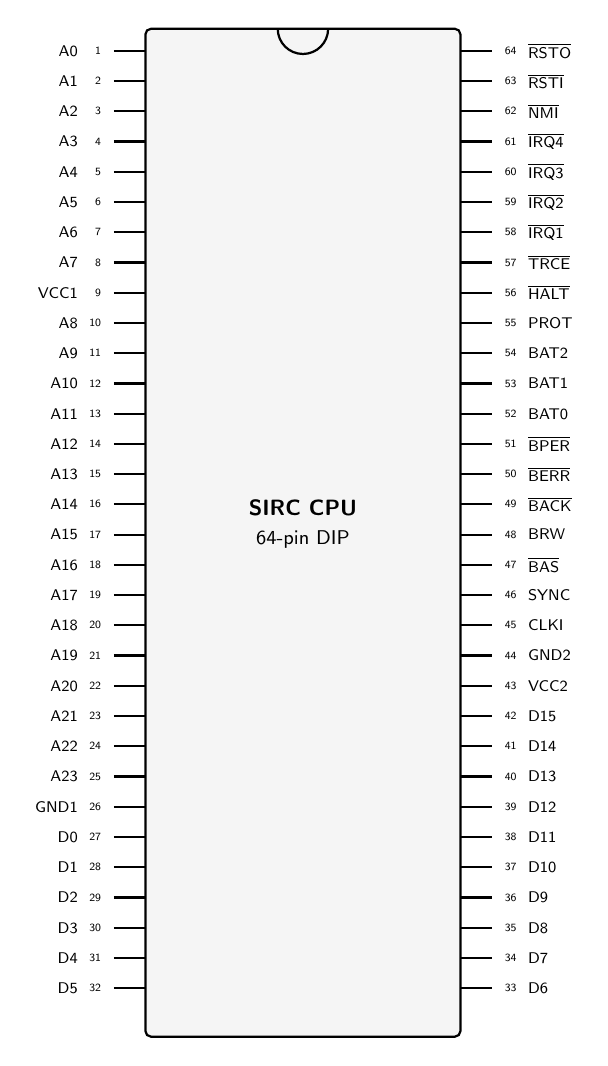
\begin{tikzpicture}[
			scale=0.8,
			transform shape,
			pinlabel/.style={font=\scriptsize},
			pinnum/.style={font=\tiny},
			body/.style={draw, thick, rounded corners=2pt, fill=gray!8},
			pin/.style={draw, thick}
		]

		% Package body
		\draw[body] (0,0) rectangle (5,-16);

		% Notch
		\draw[thick] (2.1,0) arc[start angle=180,end angle=360,radius=0.4];

		% Left-side pins: 1-32, top to bottom
		\foreach \n/\name in {
				1/A0,
				2/A1,
				3/A2,
				4/A3,
				5/A4,
				6/A5,
				7/A6,
				8/A7,
				9/VCC1,
				10/A8,
				11/A9,
				12/A10,
				13/A11,
				14/A12,
				15/A13,
				16/A14,
				17/A15,
				18/A16,
				19/A17,
				20/A18,
				21/A19,
				22/A20,
				23/A21,
				24/A22,
				25/A23,
				26/GND1,
				27/D0,
				28/D1,
				29/D2,
				30/D3,
				31/D4,
				32/D5
			} {
				\pgfmathsetmacro{\y}{-0.35 - (\n-1)*0.48}
				\draw[pin] (-0.5,\y) -- (0,\y);
				\node[pinnum, anchor=east] at (-0.58,\y) {\n};
				\node[pinlabel, anchor=east] at (-0.95,\y) {\name};
			}

		% Right-side pins: 64-33, top to bottom
		\foreach \n/\name [count=\i from 0] in {
				64/\activelow{RSTO},
				63/\activelow{RSTI},
				62/\activelow{NMI},
				61/\activelow{IRQ4},
				60/\activelow{IRQ3},
				59/\activelow{IRQ2},
				58/\activelow{IRQ1},
				57/\activelow{TRCE},
				56/\activelow{HALT},
				55/PROT,
				54/BAT2,
				53/BAT1,
				52/BAT0,
				51/\activelow{BPER},
				50/\activelow{BERR},
				49/\activelow{BACK},
				48/BRW,
				47/\activelow{BAS},
				46/SYNC,
				45/CLKI,
				44/GND2,
				43/VCC2,
				42/D15,
				41/D14,
				40/D13,
				39/D12,
				38/D11,
				37/D10,
				36/D9,
				35/D8,
				34/D7,
				33/D6
			} {
				\pgfmathsetmacro{\y}{-0.35 - \i*0.48}
				\draw[pin] (5,\y) -- (5.5,\y);
				\node[pinnum, anchor=west] at (5.58,\y) {\n};
				\node[pinlabel, anchor=west] at (5.95,\y) {\name};
			}

		% Package label
		\node[font=\bfseries] at (2.5,-7.6) {SIRC CPU};
		\node[font=\small] at (2.5,-8.1) {64-pin DIP};

	\end{tikzpicture}
	\caption{SIRC CPU 64-pin DIP Pinout, Top View}
\end{figure}

\begin{table}[H]
	\centering
	\begin{tabular}{rll}
		\toprule
		\textbf{Pin} & \textbf{Name}                      & \textbf{Description}           \\
		\midrule
		1--8         & A0--A7                             & Address bus bits 0--7          \\
		9            & VCC1                               & Power supply                   \\
		10--25       & A8--A23                            & Address bus bits 8--23         \\
		26           & GND1                               & Ground                         \\
		27--42       & D0--D15                            & Data bus bits 0--15            \\
		43           & VCC2                               & Power supply                   \\
		44           & GND2                               & Ground                         \\
		45           & CLKI                               & Clock input                    \\
		46           & SYNC                               & Instruction-sync output        \\
		47           & \activelow{BAS}                    & Bus access strobe output       \\
		48           & BRW                                & Bus read/write output          \\
		49           & \activelow{BACK}                   & Bus acknowledge input          \\
		50           & \activelow{BERR}                   & Bus error input                \\
		51           & \activelow{BPER}                   & Bus protection error input     \\
		52--54       & BAT0--BAT2                         & Bus access type bits 0--2      \\
		55           & PROT                               & Protected-mode output          \\
		56           & \activelow{HALT}                   & External CPU halt input        \\
		57           & \activelow{TRCE}                   & Force trace mode input         \\
		58--61       & \activelow{IRQ1}--\activelow{IRQ4} & Maskable interrupt inputs 1--4 \\
		62           & \activelow{NMI}                    & Non-maskable interrupt input   \\
		63           & \activelow{RSTI}                   & Reset input                    \\
		64           & \activelow{RSTO}                   & Reset output                   \\
		\bottomrule
	\end{tabular}
	\caption{SIRC CPU 64-pin DIP Pinout}
\end{table}

\chapter{Signal Descriptions}
\label{ch:signal-descriptions}

\section{Signal Conventions}

Each signal lists its own assertion convention. Address, data, and bus-type value pins use positive logic, while bus
control, handshake, interrupt, halt, trace, and reset pins generally use active-low conventions. The descriptions below
use "asserted" and "deasserted" to refer to the logical state of a signal according to its signal type.

\section{Address Bus Bits (A0--A23)}

\begin{itemize}
	\item \textbf{Direction:} Output
	\item \textbf{Signal Type:} Active High
\end{itemize}

Connected to the address bus.

These 24 pins declare the address on the bus that the CPU reads from or writes to when \activelow{BAS} (bus access
strobe) is asserted.

\section{Power Pins (VCC1--VCC2, GND1--GND2)}

These pins provide the 5~V power that the CPU requires to function.

The VCC pins must be connected to 5~V $\pm$ 5\%, and GND pins must be connected to a 0~V ground rail.

% TODO: Should I recommend some capacitors etc. to be put on the rail or something like that? Maybe should see what other CPU data sheets say
% category=Manual

\section{Data Bus Bits (D0--D15)}

\begin{itemize}
	\item \textbf{Direction:} Bidirectional
	\item \textbf{Signal Type:} Active High
\end{itemize}

Connected to the data bus.

These 16 pins are driven to a 16-bit value when the CPU is outputting to the bus, and are an input for a 16-bit value
when the CPU is reading from the bus.

\section{Clock Input (CLKI)}

\begin{itemize}
	\item \textbf{Direction:} Input
	\item \textbf{Signal Type:} Rising Edge
\end{itemize}

Progresses the CPU to the next cycle when the input transitions from low to high (rising edge).

Each rising edge of CLKI advances the CPU by one execution phase, except while a bus wait state holds the phase, while
the CPU is halted or waiting (\mnemonic{WAIT}), or while it is held in reset. With no wait states, an ordinary
instruction takes six cycles. Coprocessor calls take longer; see the Instruction Timing appendix of the \archmanual{}.

\section{Instruction Sync Output (SYNC)}

\begin{itemize}
	\item \textbf{Direction:} Output
	\item \textbf{Signal Type:} Active High
\end{itemize}

Asserted only at phase 0 of an instruction fetch or of an exception-unit dispatch slot. It remains asserted if a wait
state holds that phase. It is deasserted in every other phase, in every other coprocessor slot (DMA and maths), in
every DMA continuation slot, and while the CPU is halted, waiting, or in reset.

This pin is useful for debugging.

\section{Bus Access Strobe Output (BAS)}

\begin{itemize}
	\item \textbf{Direction:} Output
	\item \textbf{Signal Type:} Active Low
\end{itemize}

When the CPU is ready to perform a bus operation, \activelow{BAS} is asserted after the address pins, BRW, BAT, PROT,
and any CPU-driven data pins are valid.

\activelow{BAS} remains asserted until the bus responds with \activelow{BACK}, \activelow{BERR}, or \activelow{BPER}. If no response is asserted, the CPU holds the
current execution phase and repeats the same bus request on the following clock.

\section{Bus Read/Write Output (BRW)}

\begin{itemize}
	\item \textbf{Direction:} Output
	\item \textbf{Signal Type:} Read High / Write Low
\end{itemize}

Only relevant when the \activelow{BAS} (Bus access strobe output) is asserted.

When high, the CPU is requesting a read from the bus. When low, the CPU is requesting a write to the bus.

\section{Bus Acknowledge Input (BACK)}

\begin{itemize}
	\item \textbf{Direction:} Input
	\item \textbf{Signal Type:} Active Low
\end{itemize}

When asserted, the bus is reporting that the requested read/write completed successfully. On reads, the CPU samples
D0--D15 on the clock edge that accepts \activelow{BACK}.

If all bus devices are fast and can complete reads/writes in a single cycle, this pin can be permanently held asserted.

\section{Bus Error Input (BERR)}

\begin{itemize}
	\item \textbf{Direction:} Input
	\item \textbf{Signal Type:} Active Low
\end{itemize}

When asserted, the bus is reporting that the requested read/write was unsuccessful.

This causes the CPU to abort the I/O operation and raise a bus fault exception, except during an exception-vector
fetch. The response to a failed vector fetch is described in the Exception and Interrupt Handling chapter of the
\archmanual{}: a failed fault-vector fetch raises a double fault, and a failed reset-vector fetch re-enters reset.

For example, a bus error might be raised by I/O to an address that is not connected to any device.

\section{Bus Protection Error Input (BPER)}

\begin{itemize}
	\item \textbf{Direction:} Input
	\item \textbf{Signal Type:} Active Low
\end{itemize}

When asserted, the bus is reporting that the requested read/write was to a valid address/device, but that the I/O is
disallowed given the current state of the CPU or bus.

This causes the CPU to abort the I/O operation and raise a bus protection fault exception, except during an
exception-vector fetch. The response to a failed vector fetch is described in the Exception and Interrupt Handling
chapter of the \archmanual{}: a failed fault-vector fetch raises a double fault, and a failed reset-vector fetch
re-enters reset.

It behaves much like the \activelow{BERR} pin but raises a different fault so that programs can handle it differently.

For example, a bus protection error might be raised by a write to ROM, or by a write to a privileged section of memory
when the CPU is not in supervisor mode.

\section{Bus Access Type Bits (BAT0--BAT2)}

\begin{itemize}
	\item \textbf{Direction:} Output
	\item \textbf{Signal Type:} Active High
\end{itemize}

Output by the CPU to describe what I/O operation it is performing.

These pins can provide hints to external devices during I/O.

For example, if a memory controller knows that the DMA coprocessor will be reading more than one sequential address, it
can prefetch the next address.

Another example is a memory controller providing memory protection when these pins are used with the PROT
(Protected-mode output) pin. A memory controller might assert \activelow{BPER} (bus protection error) if BAT is 010
(data read), PROT is 1 (protected mode) and the address is in a protected memory region.

\begin{table}[H]
	\centering
	\begin{tabular}{rrrl}
		\toprule
		\textbf{BAT2} & \textbf{BAT1} & \textbf{BAT0} & \textbf{Description}        \\
		\midrule
		0             & 0             & 0             & No I/O                      \\
		0             & 0             & 1             & Instruction Fetch           \\
		0             & 1             & 0             & Data Read                   \\
		0             & 1             & 1             & Data Write                  \\
		1             & 0             & 0             & Exception Vector Fetch      \\
		1             & 0             & 1             & DMA Coprocessor Read Burst  \\
		1             & 1             & 0             & DMA Coprocessor Write Burst \\
		1             & 1             & 1             & Reserved                    \\
		\bottomrule
	\end{tabular}
	\caption{Bus Access Type Bits Meaning}
\end{table}

\section{Protected-Mode Output (PROT)}

\begin{itemize}
	\item \textbf{Direction:} Output
	\item \textbf{Signal Type:} Active High
\end{itemize}

Indicates whether the CPU is in protected mode (high) or in supervisor mode (low).

Follows the status register Protected Mode (P) bit, except that it is deasserted for every exception-vector fetch (BAT
100), which is a supervisor access even when the exception is taken from protected mode.

When the CPU is in protected mode, programs have access to fewer types of instructions, for example they cannot write
to the high word of the address registers.

Exposing this as an external pin allows other devices such as memory controllers to block access to protected regions
of memory by raising bus protection errors.

\section{External CPU Halt Input (HALT)}

\begin{itemize}
	\item \textbf{Direction:} Input
	\item \textbf{Signal Type:} Active Low
\end{itemize}

When asserted, the CPU stops executing instructions.

\activelow{HALT} is sampled at every phase 0. If it is asserted there, the CPU stops at that phase 0 with the bus idle. The halt
can occur between an instruction and its coprocessor dispatch slot, between DMA slots, or before a fault, interrupt, or
reset dispatch. Halt latency is at most six cycles. The CPU performs no bus cycles while halted. The interrupt lines
are still sampled and a Level 5 edge is still latched, but nothing is dispatched until the CPU resumes. The CPU resumes
exactly where it stopped when the input is deasserted. A reset ends the halt, but if \activelow{HALT} is still asserted after
reset, the CPU halts at the first phase 0, before the reset-vector fetch.

This pin is useful for hardware-driven debugging, as the CPU can be halted and the state of the system examined.

\section{Force Trace Mode Input (TRCE)}

\begin{itemize}
	\item \textbf{Direction:} Input
	\item \textbf{Signal Type:} Active Low
\end{itemize}

When asserted at an instruction boundary, the instruction being started is traced regardless of whether software has
cleared the Trace Mode (T) flag in the status register. No trace fault is raised while a fault handler runs (exception
level 7), since it would escalate to a double fault.

In trace mode, the CPU raises an exception on every instruction to allow software debugging.

\section{Maskable Interrupt Inputs (IRQ1--IRQ4)}

\begin{itemize}
	\item \textbf{Direction:} Input
	\item \textbf{Signal Type:} Active Low
\end{itemize}

When asserted, the corresponding hardware interrupt line is sampled by the CPU.

The lines can be masked by the Hardware Interrupt Enable Bits (E1--E4) of the status register.

Interrupt inputs are level-sensitive. They are sampled on every clock cycle except during reset: from the cycle in
which reset is requested until the reset-vector fetch completes, no interrupt line, including \activelow{NMI}, is
sampled. Enabled interrupt lines are latched in the pending hardware-exceptions register; disabled maskable lines are
ignored and not queued, and a line is not latched while its own handler or a higher-priority one is running. The
requesting device must hold the line asserted until its handler acknowledges it; an assertion withdrawn before it is
latched is not recognized. If an interrupt pin remains asserted after its handler returns, it may be sampled again
through the normal interrupt rules.

See the Exception and Interrupt Handling chapter of the \archmanual{} for more details.

\section{Non-Maskable Interrupt Inputs (NMI)}

\begin{itemize}
	\item \textbf{Direction:} Input
	\item \textbf{Signal Type:} Active Low
\end{itemize}

When asserted, the CPU samples the Level 5 hardware exception line. Unlike \activelow{IRQ1}--\activelow{IRQ4}, which
are level-sensitive, \activelow{NMI} is edge-triggered: it fires once on assertion regardless of how long the pin is
held, and the pin must be released and reasserted to fire again. An \activelow{NMI} held asserted across a reset does
not fire afterward, because reset does not clear the edge detector's last sampled level and so no transition occurs;
the pin must be released and reasserted.

This interrupt cannot be masked. A new assertion of this pin (a fresh edge) while a Level 5 handler is running raises a
Level Five Hardware Exception Conflict fault; holding the pin asserted from the edge that started the handler does not.
A further edge while a Level 5 request is still pending (for example, behind a fault handler) is lost and is reported
by a single conflict fault when Level 5 is next selected.

Because \activelow{NMI} is edge-triggered, holding the pin asserted after its handler returns does not by itself cause
it to fire again. The pin must be released (driven high) for at least one CLKI cycle and asserted (driven low) again;
the request fires on the clock edge at which the assertion is first sampled. Level 5 exception handlers must therefore
execute quickly, and \activelow{NMI} should be asserted only for important, non-interruptible events.

\section{Reset Input (RSTI)}

\begin{itemize}
	\item \textbf{Direction:} Input
	\item \textbf{Signal Type:} Active Low
\end{itemize}

External devices can use this pin to force a reset of the CPU.

When asserted, the CPU immediately aborts the current instruction or bus wait, stops normal processing, resets to phase
0, and begins the reset sequence described in the Exception and Interrupt Handling chapter of the \archmanual{}.

The \activelow{RSTO} pin is also asserted.

The reset-output hold is six CLKI cycles. The cycle in which \activelow{RSTI} is first sampled asserted counts as the
first, and \activelow{RSTO} stays asserted for five further cycles after \activelow{RSTI} is sampled deasserted, so an
\activelow{RSTI} assertion of $n$ cycles gives $n + 5$ cycles of \activelow{RSTO}. A software reset and a reset-vector
fetch retry each give a six-cycle hold.

When this pin is deasserted, the CPU completes the reset-output hold, stops asserting the \activelow{RSTO} pin, and the
exception unit fetches the reset vector.

If a system needs external devices to be reset for longer than the CPU reset-output hold, reset timing must be managed
externally to the CPU, and \activelow{RSTI} must remain asserted for as long as the other devices need to reset.

\section{Reset Output (RSTO)}

\begin{itemize}
	\item \textbf{Direction:} Output
	\item \textbf{Signal Type:} Active Low
\end{itemize}

Asserted while the \activelow{RSTI} pin is asserted and during the reset-output hold before reset-vector fetch.

It is also asserted for the reset-output hold after a software reset, after a reset caused by a failed double-fault
vector fetch, and for a further hold before the CPU retries a reset-vector fetch that failed. Each of these holds is
six CLKI cycles. A reset caused by a failed double-fault vector fetch behaves as a software reset: the six-cycle
\activelow{RSTO} hold is followed by the reset-vector fetch.

A reset can be triggered by asserting the Reset input (\activelow{RSTI}) pin, or in software by the exception
coprocessor meta-instruction \mnemonic{RSET}.

This pin is useful to reset other devices on the bus whenever the CPU is reset or to trigger more complex reset/boot
controllers.

\chapter{Bus Interface}
\label{ch:bus-interface}

\section{Clocked Bus Model}
\label{sec:clocked-bus-model}

All bus timing is described relative to the rising edge of CLKI. The CPU presents a bus request during the execution
phase that needs external access. If no response is asserted, the CPU repeats the same request and does not advance to
the next execution phase.

A no-wait-state bus access assumes that the selected external device can assert \activelow{BACK} and, for reads, drive
valid data during the same CLKI interval in which \activelow{BAS} is asserted, so the CPU accepts the transfer on the
next rising edge. A device that samples the request on one clock edge and cannot return \activelow{BACK} or read data
until a later edge adds wait states; this is the normal way to attach slower synchronous memory or peripherals.

\begin{table}[H]
	\centering
	\small
	\begin{tabularx}{\textwidth}{lX}
		\toprule
		\textbf{Signal} & \textbf{Timing rule}                                                                                                                                                                                                                                                                                          \\
		\midrule
		A0--A23         & Valid whenever \activelow{BAS} is asserted. Stable until the request completes or aborts.                                                                                                                                                                                                                     \\
		D0--D15         & Driven by the CPU only for writes. On reads, the selected device drives the bus and the CPU samples D0--D15 when \activelow{BACK} is accepted.                                                                                                                                                                \\
		BRW             & Valid whenever \activelow{BAS} is asserted. High requests a read; low requests a write. Stable until the request completes or aborts.                                                                                                                                                                         \\
		BAT0--BAT2      & Valid whenever \activelow{BAS} is asserted. Encodes the access type for the active request and is stable until completion or abort.                                                                                                                                                                           \\
		PROT            & Reflects the status register P bit, except that it is deasserted for exception-vector fetches, and may be used with \activelow{BAS}, BAT, and A0--A23 by external protection logic.                                                                                                                           \\
		\activelow{BAS} & Asserted while a bus request is active. Remains asserted across wait states.                                                                                                                                                                                                                                  \\
		SYNC            & Asserted only at phase 0 of an instruction fetch or of an exception-unit dispatch slot, and remains asserted if a wait state holds that phase. Deasserted in every other phase, in every other coprocessor slot (DMA and maths) and DMA continuation slot, and while the CPU is halted, waiting, or in reset. \\
		\bottomrule
	\end{tabularx}
	\caption{CPU Bus Output Timing Rules}
	\label{tab:bus-output-timing-rules}
\end{table}

When \activelow{BAS} is deasserted there is no active bus cycle. External devices must ignore A0--A23, D0--D15, BRW,
and BAT0--BAT2 unless \activelow{BAS} is asserted.

The CPU keeps driving A0--A23, BRW, and BAT0--BAT2 while \activelow{BAS} is deasserted, including while it is halted,
waiting (\mnemonic{WAIT}), or in reset. BRW is high and BAT0--BAT2 is 000 (No I/O); this is the idle value. The value
of A0--A23 while idle is architecturally undefined. The SIRC-1 has no bus-release mechanism: the CPU never three-states
these signals, and \activelow{HALT} does not free the bus for another master.

\section{Bus Cycle Completion}

\begin{table}[H]
	\centering
	\small
	\begin{tabularx}{\textwidth}{lX}
		\toprule
		\textbf{Response} & \textbf{Effect When Sampled While \activelow{BAS} Is Asserted}                                                                                                 \\
		\midrule
		\activelow{BACK}  & Completes the request successfully. For reads, D0--D15 is sampled on the accepting clock edge. For writes, the write is externally committed.                  \\
		\activelow{BERR}  & Aborts the request and raises a bus fault. Read data is ignored and the CPU does not consider a write successfully committed.                                  \\
		\activelow{BPER}  & Aborts the request and raises a bus protection fault. Read data is ignored and the CPU does not consider a write successfully committed.                       \\
		No response       & Inserts a wait state. The CPU remains in the current execution phase and keeps A0--A23, D0--D15 for writes, BRW, BAT0--BAT2, PROT, and \activelow{BAS} stable. \\
		\bottomrule
	\end{tabularx}
	\caption{Bus Response Timing Rules}
	\label{tab:bus-response-timing-rules}
\end{table}

A bus cycle terminated by Bus Error or Bus Protection Error is architecturally unsuccessful. An external device must
not commit any externally visible effect from a bus cycle for which it asserts the corresponding error signal. For a
write, the device must not act on the data driven to it. For a read, the device must not cause any side effect that the
access would otherwise have, for example a status register that clears on read. This is what makes Bus Fault and Bus
Protection Fault safe to retry (see the Exception and Interrupt Handling chapter of the \archmanual{}): the CPU assumes
that a bus cycle it aborted with one of these signals never happened.

\activelow{BACK}, \activelow{BERR}, and \activelow{BPER} are logically mutually exclusive. If more than one is
asserted for the same request, \activelow{BERR} has priority, then \activelow{BPER}, then \activelow{BACK}.

\section{Bus Cycle Types}

\begin{table}[H]
	\centering
	\small
	\begin{tabularx}{\textwidth}{lXXX}
		\toprule
		\textbf{Cycle} & \textbf{CPU drives}                                 & \textbf{External device drives}      & \textbf{Completion}                                                                  \\
		\midrule
		Read           & A0--A23, BRW=1, BAT, \activelow{BAS}, PROT          & D0--D15 for the selected address     & \activelow{BACK} samples data; \activelow{BERR}/\activelow{BPER} aborts.             \\
		Write          & A0--A23, D0--D15, BRW=0, BAT, \activelow{BAS}, PROT & No data bus drive                    & \activelow{BACK} accepts write; \activelow{BERR}/\activelow{BPER} aborts.            \\
		Wait state     & Same values as the previous request cycle           & Same ownership as the active request & Continues until \activelow{BACK}, \activelow{BERR}, or \activelow{BPER} is asserted. \\
		No bus cycle   & No active bus cycle                                 & No device drives D0--D15             & CPU advances internally.                                                             \\
		\bottomrule
	\end{tabularx}
	\caption{External Bus Cycle Ownership}
	\label{tab:bus-cycle-ownership}
\end{table}

\section{DMA Bus Cycles}
\label{sec:dma-bus-cycles}

The optional DMA coprocessor performs bulk word transfers as ordinary single-word bus cycles. This section describes
what an external device observes; the \archmanual{} describes the commands and their timing in the Coprocessor
Instructions chapter. A CPU model without the DMA coprocessor never drives BAT 101 or 110.

\begin{itemize}
	\item Phase 0 of the DMA slot is a setup cycle with no bus access: \activelow{BAS} is deasserted and the idle values of
	      Section~\ref{sec:clocked-bus-model} apply.
	\item From phase 1, each DMA access is a separate bus cycle. \activelow{BAS} is asserted for the access, and the access is
	      completed by its own \activelow{BACK}, \activelow{BERR}, or \activelow{BPER}, exactly as for any other bus cycle.
	\item Addresses ascend by one word per access, for both positive and negative counts.
	\item BAT is 101 (DMA coprocessor read burst) for reads and 110 (DMA coprocessor write burst) for writes. BRW is high for
	      reads and low for writes. A DMA read command uses only reads and a DMA write command uses only writes. A DMA copy
	      command reads a chunk of up to seven words with BAT 101, then writes the chunk with BAT 110.
	\item PROT follows the status register P bit, as for any other access.
	\item SYNC is deasserted throughout the DMA slot and every DMA continuation slot.
	\item A wait state on a DMA access holds the phase and keeps the access signals stable, as for any other bus cycle. Each wait
	      state adds exactly one cycle to the transfer.
\end{itemize}

Figure~\ref{fig:dma-read-timing} shows a three-word DMA read with no wait states. The address labels \texttt{start},
\texttt{start+1}, and \texttt{start+2} are the first, second, and third word addresses of the transfer in ascending
order.

\begin{figure}[H]
	\centering
	\small
	\begin{tikztimingtable}[sirc timing diagram]
		CLKI                         & 6{C}                                            \\
		Phase                        & D{Setup} D{Read 1} D{Read 2} D{Read 3} D{} D{}  \\
		SYNC                         & L L L L L L                                     \\
		\activelow{BAS}              & H L L L H H                                     \\
		BRW                          & H H H H H H                                     \\
		BAT0--BAT2                   & D{None} D{101} D{101} D{101} D{None} D{None}    \\
		A0--A23                      & D{} D{start} D{start+1} D{start+2} D{} D{}      \\
		D0--D15                      & Z D{d0} D{d1} D{d2} Z Z                         \\
		\activelow{BACK}             & H L L L H H                                     \\
		\activelow{BERR}/\activelow{BPER} & H H H H H H                                \\
	\end{tikztimingtable}
	\caption{Three-Word DMA Read with No Wait States}
	\label{fig:dma-read-timing}
\end{figure}

\section{Control Input Sampling}

\begin{table}[H]
	\centering
	\small
	\begin{tabularx}{\textwidth}{lX}
		\toprule
		\textbf{Input}                                       & \textbf{Sampling rule}                                                                                                                                                                                                                                                                                                                                                                  \\
		\midrule
		\activelow{BACK}, \activelow{BERR}, \activelow{BPER} & Sampled while \activelow{BAS} is asserted. They complete or abort the active bus request.                                                                                                                                                                                                                                                                                               \\
		\activelow{IRQ1}--\activelow{IRQ4}                   & Level-sensitive and sampled every cycle, except during reset. The requesting device must hold the line asserted until its handler acknowledges it; a line is not latched while its own or a higher-priority handler runs. From the cycle in which reset is requested until the reset-vector fetch completes, no interrupt line, including \activelow{NMI}, is sampled.                  \\
		\activelow{NMI}                                      & Edge-triggered. Fires once on assertion regardless of how long the pin is held; the pin must be released and reasserted to fire again.                                                                                                                                                                                                                                                  \\
		\activelow{HALT}                                     & Sampled at every phase 0. If asserted, the CPU stops at that phase 0 with the bus idle, which can fall between an instruction and its coprocessor dispatch slot, between DMA slots, or before a fault, interrupt, or reset dispatch. Halt latency is at most six cycles. The CPU resumes where it stopped when the input is deasserted; interrupt lines are still sampled while halted. \\
		\activelow{TRCE}                                     & Sampled at instruction boundaries. If asserted, the instruction being started is traced, except inside a fault handler.                                                                                                                                                                                                                                                                 \\
		\activelow{RSTI}                                     & May be asserted at any time. It aborts the current instruction, exception dispatch, or bus wait and starts the reset sequence.                                                                                                                                                                                                                                                          \\
		\bottomrule
	\end{tabularx}
	\caption{External Input Sampling Rules}
	\label{tab:external-input-sampling-rules}
\end{table}

\chapter{Bus Timing Diagrams}
\label{ch:bus-timing}

\section{Bus Cycle Diagrams}

The timing diagrams below show cycle-level logical timing. Each labeled interval represents one CLKI cycle as observed
between rising edges. Waveform rows show physical logic levels; for active-low signals, \texttt{L} means asserted and
\texttt{H} means deasserted. Address, data, \texttt{BAT}, and phase rows are value bands rather than electrical
setup/hold specifications. An empty band means that the row carries no defined value in that cycle. Every cycle begins
with a CLKI rising edge. The pulses in the \texttt{Sample} row mark the rising edges at which the CPU samples
\activelow{BACK}, \activelow{BERR}, \activelow{BPER}, and read data, which are the edges that end the cycles in which
\activelow{BAS} is asserted (Section~\ref{sec:clock-edges}).

Table~\ref{tab:figure-phase-labels} lists the labels used in the phase bands, which name the activity of each cycle.

\begin{table}[H]
	\centering
	\begin{tabularx}{\textwidth}{@{}p{4.2cm}X@{}}
		\toprule
		\textbf{Label}                                                         & \textbf{Meaning}                                                                                                                                  \\
		\midrule
		\texttt{IF high}, \texttt{IF low}                                      & The high-word and low-word instruction-fetch cycles (phases 0 and 1).                                                                             \\
		\texttt{Decode}, \texttt{Execute}, \texttt{Memory}, \texttt{Writeback} & Phases 2, 3, 4 and 5 of an instruction. Section~\ref{sec:execution-phases} defines the phases; no other definition is needed to read the figures. \\
		\texttt{EA}                                                            & The effective-address calculation cycle.                                                                                                          \\
		\texttt{EV high}, \texttt{EV low}                                      & The high-word and low-word cycles of an exception-vector fetch.                                                                                   \\
		\texttt{RV high}, \texttt{RV low}                                      & The high-word and low-word cycles of the reset-vector fetch.                                                                                      \\
		\texttt{Mem}                                                           & The data-access cycle of a load or store.                                                                                                         \\
		\texttt{next}                                                          & The cycle that follows a bus transfer, in which the bus is idle.                                                                                  \\
		\texttt{req}                                                           & In a wait-state figure, the cycle in which the request is first presented.                                                                        \\
		\texttt{wait}                                                          & A cycle in which no response is yet asserted.                                                                                                     \\
		\texttt{done}                                                          & The cycle in which the response completes the transfer.                                                                                           \\
		\texttt{Prev WB}                                                       & The writeback phase of the preceding instruction.                                                                                                 \\
		\texttt{Enter}                                                         & The first cycle of exception entry after the vector is fetched.                                                                                   \\
		\texttt{reset}                                                         & The cycle in which \activelow{RSTI} is first sampled asserted.                                                                                    \\
		\texttt{hold}                                                          & A cycle of the reset-output hold.                                                                                                                 \\
		\texttt{BERR}, \texttt{BPER}                                           & The abort cases.                                                                                                                                  \\
		\bottomrule
	\end{tabularx}
	\caption{Phase Band Labels in the Timing Diagrams}
	\label{tab:figure-phase-labels}
\end{table}

\texttt{BAT} bands name the bus-access type. The diagrams use \texttt{IF} for instruction fetch, \texttt{DR} for data
read, \texttt{DW} for data write, \texttt{EV} for exception vector fetch of vector $n$ at word addresses $2n$ and
$2n+1$, and \texttt{None} for no bus access. \texttt{active} is the type of the access in progress when the abort is
signalled. Address bands show \texttt{PC} and \texttt{PC+1} for the fetch addresses, \texttt{EA} for the effective
address, and \texttt{addr} for the address of the access in progress. Data bands show the \texttt{high} or \texttt{low}
word of a two-word transfer, or \texttt{data} for a single-word transfer.

\begin{figure}[H]
	\centering
	\small
	\begin{tikztimingtable}[sirc timing diagram]
		CLKI        & L 3{0.5H 0.5L}                         \\
		Phase       & D{IF high} D{IF low} D{Decode} D{} \\
		SYNC        & H L L L                       \\
		\activelow{BAS}         & L L H H                       \\
		BRW         & H H H H                       \\
		BAT0--BAT2  & D{IF} D{IF} D{None} D{None}   \\
		A0--A23     & D{PC} D{PC+1} D{} D{}         \\
		D0--D15     & D{high} D{low} Z Z            \\
		\activelow{BACK}        & L L H H                       \\
		\activelow{BERR}/\activelow{BPER}   & H H H H                       \\
		Sample      & 0.95L 0.1H 0.9L 0.1H 1.95L \\
	\end{tikztimingtable}
	\caption{Instruction-Fetch High-Word and Low-Word Reads with No Wait States}
	\label{fig:instruction-fetch-read-timing}
\end{figure}

\begin{figure}[H]
	\centering
	\small
	\begin{tikztimingtable}[sirc timing diagram]
		CLKI        & L 2{0.5H 0.5L}                      \\
		Phase       & D{Mem} D{next} D{}        \\
		SYNC        & L L L                     \\
		\activelow{BAS}         & L H H                     \\
		BRW         & H H H                     \\
		BAT0--BAT2  & D{DR} D{None} D{None}     \\
		A0--A23     & D{EA} D{} D{}             \\
		D0--D15     & D{data} Z Z               \\
		\activelow{BACK}        & L H H                     \\
		\activelow{BERR}/\activelow{BPER}   & H H H                     \\
		Sample      & 0.95L 0.1H 1.95L \\
	\end{tikztimingtable}
	\caption{Data Read Cycle with No Wait State}
	\label{fig:data-read-timing}
\end{figure}

\begin{figure}[H]
	\centering
	\small
	\begin{tikztimingtable}[sirc timing diagram]
		CLKI        & L 2{0.5H 0.5L}                       \\
		Phase       & D{Mem} D{next} D{}         \\
		SYNC        & L L L                      \\
		\activelow{BAS}         & L H H                      \\
		BRW         & L H H                      \\
		BAT0--BAT2  & D{DW} D{None} D{None}      \\
		A0--A23     & D{EA} D{} D{}              \\
		D0--D15     & D{data} Z Z                \\
		\activelow{BACK}        & L H H                      \\
		\activelow{BERR}/\activelow{BPER}   & H H H                      \\
		Sample      & 0.95L 0.1H 1.95L \\
	\end{tikztimingtable}
	\caption{Data Write Cycle with No Wait State}
	\label{fig:data-write-timing}
\end{figure}

\begin{figure}[H]
	\centering
	\small
	\begin{tikztimingtable}[sirc timing diagram]
		CLKI        & L 3{0.5H 0.5L}                                 \\
		Phase       & D{EV high} D{EV low} D{next} D{} \\
		SYNC        & H L L L                              \\
		\activelow{BAS}         & L L H H                              \\
		BRW         & H H H H                              \\
		BAT0--BAT2  & D{EV} D{EV} D{None} D{None}          \\
		A0--A23     & D{$2n$} D{$2n+1$} D{} D{}            \\
		D0--D15     & D{high} D{low} Z Z                   \\
		\activelow{BACK}        & L L H H                              \\
		\activelow{BERR}/\activelow{BPER}   & H H H H                              \\
		Sample      & 0.95L 0.1H 0.9L 0.1H 1.95L \\
	\end{tikztimingtable}
	\caption{Exception-Vector Fetch with High-Word Then Low-Word Reads}
	\label{fig:exception-vector-fetch-timing}
\end{figure}

\begin{figure}[H]
	\centering
	\small
	\begin{tikztimingtable}[sirc timing diagram]
		CLKI        & L 3{0.5H 0.5L}                              \\
		Phase       & D{req} D{wait} D{done} D{next}        \\
		SYNC        & L L L L                           \\
		\activelow{BAS}         & L L L H                           \\
		BRW         & H H H H                           \\
		BAT0--BAT2  & D{DR} D{DR} D{DR} D{None}           \\
		A0--A23     & D{addr} D{addr} D{addr} D{}         \\
		D0--D15     & Z Z D{data} Z                       \\
		\activelow{BACK}        & H H L H                           \\
		\activelow{BERR}/\activelow{BPER}   & H H H H                           \\
		Sample      & 0.95L 0.1H 0.9L 0.1H 0.9L 0.1H 0.95L \\
	\end{tikztimingtable}
	\caption{Wait-State Insertion when No Bus Response Is Asserted}
	\label{fig:bus-wait-state-timing}
\end{figure}

\begin{figure}[H]
	\centering
	\small
	\begin{tikztimingtable}[sirc timing diagram]
		CLKI        & L 3{0.5H 0.5L}                          \\
		Case        & D{BERR} D{} D{BPER} D{}             \\
		\activelow{BAS}         & L H L H                       \\
		BRW         & H H H H                       \\
		\activelow{BACK}        & H H H H                       \\
		\activelow{BERR}        & L H H H                       \\
		\activelow{BPER}        & H H L H                       \\
		BAT0--BAT2  & D{active} D{None} D{active} D{None} \\
		A0--A23     & D{addr} D{} D{addr} D{}             \\
		D0--D15     & Z Z Z Z                       \\
		Sample      & 0.95L 0.1H 1.9L 0.1H 0.95L \\
	\end{tikztimingtable}
	\caption{Bus-Error and Bus-Protection Abort Timing}
	\label{fig:bus-abort-timing}
\end{figure}

\begin{figure}[H]
	\centering
	\small
	\begin{tikztimingtable}[sirc timing diagram]
		CLKI        & L 5{0.5H 0.5L}                                      \\
		Phase       & D{IF high} D{IF low} D{Decode} D{Execute} D{Memory} D{Writeback} \\
		SYNC        & H L L L L L                                \\
		\activelow{BAS}         & L L H H H H                                \\
		BRW         & H H H H H H                                \\
		BAT0--BAT2  & D{IF} D{IF} D{None} D{None} D{None} D{None} \\
		A0--A23     & D{PC} D{PC+1} D{} D{} D{} D{}              \\
		D0--D15     & D{high} D{low} Z Z Z Z                     \\
		\activelow{BACK}        & L L H H H H                                \\
		\activelow{BERR}/\activelow{BPER}   & H H H H H H                                \\
		Sample      & 0.95L 0.1H 0.9L 0.1H 3.95L \\
	\end{tikztimingtable}
	\caption{Complete Register-Only ALU Instruction with No Wait States}
	\label{fig:alu-instruction-cycle-timing}
\end{figure}

\begin{figure}[H]
	\centering
	\small
	\begin{tikztimingtable}[sirc timing diagram]
		CLKI        & L 5{0.5H 0.5L}                                      \\
		Phase       & D{IF high} D{IF low} D{Decode} D{EA} D{Memory} D{Writeback} \\
		SYNC        & H L L L L L                                \\
		\activelow{BAS}         & L L H H L H                                \\
		BRW         & H H H H H H                                \\
		BAT0--BAT2  & D{IF} D{IF} D{None} D{None} D{DR} D{None}  \\
		A0--A23     & D{PC} D{PC+1} D{} D{} D{EA} D{}            \\
		D0--D15     & D{high} D{low} Z Z D{data} Z               \\
		\activelow{BACK}        & L L H H L H                                \\
		\activelow{BERR}/\activelow{BPER}   & H H H H H H                                \\
		Sample      & 0.95L 0.1H 0.9L 0.1H 2.9L 0.1H 0.95L \\
	\end{tikztimingtable}
	\caption{Complete LOAD Instruction with No Wait States}
	\label{fig:load-instruction-cycle-timing}
\end{figure}

\section{Reset and Interrupt Timing Examples}

Figure~\ref{fig:hardware-reset-cycle-timing} shows a hardware reset in which \activelow{RSTI} is asserted for one
clock. The reset-output hold is six CLKI cycles in this case. The cycle in which \activelow{RSTI} is first sampled
asserted counts as the first, and \activelow{RSTO} stays asserted for five further cycles after \activelow{RSTI} is
sampled deasserted. An \activelow{RSTI} assertion of $n$ cycles therefore gives $n + 5$ cycles of \activelow{RSTO}. A
software reset and a reset-vector fetch retry each give a six-cycle hold. The reset-vector fetch does not begin until
\activelow{RSTI} is deasserted and the reset-output hold has completed.

\begin{figure}[H]
	\centering
	\small
	\begin{tikztimingtable}[sirc timing diagram]
		CLKI        & L 7{0.5H 0.5L}                                         \\
		Phase       & D{reset} D{hold} D{hold} D{hold} D{hold} D{hold} D{RV high} D{RV low} \\
		\activelow{RSTI}        & L H H H H H H H                               \\
		\activelow{RSTO}        & L L L L L L H H                               \\
		\activelow{BAS}         & H H H H H H L L                               \\
		BRW         & H H H H H H H H                               \\
		BAT0--BAT2  & D{None} D{None} D{None} D{None} D{None} D{None} D{EV} D{EV} \\
		A0--A23     & D{} D{} D{} D{} D{} D{} D{0} D{1}     \\
		D0--D15     & Z Z Z Z Z Z D{high} D{low}                    \\
		\activelow{BACK}        & H H H H H H L L                               \\
		\activelow{BERR}/\activelow{BPER}   & H H H H H H H H                               \\
		Sample      & 6.95L 0.1H 0.9L 0.05H \\
	\end{tikztimingtable}
	\caption{Hardware Reset with One-Cycle \activelow{RSTI} Assertion and Reset-Vector Fetch}
	\label{fig:hardware-reset-cycle-timing}
\end{figure}

Figure~\ref{fig:irq-sampling-cycle-timing} shows an enabled maskable interrupt asserted before an instruction boundary.
The CPU samples the interrupt lines on every clock cycle, so the request is latched in the cycle it is first seen, but
it is dispatched only at the next phase 0 at which no coprocessor call or command is pending or active. A request first
sampled at the rising edge that starts phase 0 is dispatched in that phase 0. The following exception-unit dispatch
fetches the selected hardware-interrupt vector instead of fetching the next processing-unit instruction. A request
latched partway through an instruction waits for the next such phase 0. The figure holds
\activelow{IRQ1}--\activelow{IRQ4} asserted throughout because the requesting device must hold the line asserted until
its handler acknowledges it.

\begin{figure}[H]
	\centering
	\small
	\begin{tikztimingtable}[sirc timing diagram]
		CLKI        & L 4{0.5H 0.5L}                                  \\
		Phase       & D{Prev WB} D{EV high} D{EV low} D{Decode} D{Enter} \\
		\activelow{IRQ1}--\activelow{IRQ4}  & L L L L L                              \\
		SYNC        & L H L L L                              \\
		\activelow{BAS}         & H L L H H                              \\
		BRW         & H H H H H                              \\
		BAT0--BAT2  & D{None} D{EV} D{EV} D{None} D{None}    \\
		A0--A23     & D{} D{$2n$} D{$2n+1$} D{} D{}          \\
		D0--D15     & Z D{high} D{low} Z Z                   \\
		\activelow{BACK}        & H L L H H                              \\
		\activelow{BERR}/\activelow{BPER}   & H H H H H                              \\
		Sample      & 1.95L 0.1H 0.9L 0.1H 1.95L \\
	\end{tikztimingtable}
	\caption{Enabled \activelow{IRQ} Latched Before an Instruction Boundary and Dispatched with No Wait States}
	\label{fig:irq-sampling-cycle-timing}
\end{figure}

\chapter{Electrical Characteristics}
\label{ch:electrical-characteristics}

The only electrical requirement currently specified is the supply: \texttt{VCC1} and \texttt{VCC2} must be connected to
5~V $\pm$ 5\% and \texttt{GND1} and \texttt{GND2} to the 0~V rail (see Chapter~\ref{ch:signal-descriptions}).

The bus timing in this manual is cycle-level logical timing, measured in \texttt{CLKI} cycles. The following
characteristics have not yet been specified and will be added to this chapter when they are:

\begin{itemize}
	\item Input and output voltage levels
	\item Clock frequency range
	\item Setup, hold and propagation delay times
	\item Fanout and maximum board loading
	\item Supply current and power dissipation
	\item Package dimensions and thermal characteristics
\end{itemize}

Until then, designs must not assume any value for these characteristics.


\backmatter

\clearpage
\thispagestyle{empty}
\begin{center}

	\vspace*{1.5cm}

	{\Large\bfseries SIRC-1 Hardware Reference Manual}

	\vspace{1cm}

	\begin{minipage}{0.8\textwidth}
		This manual describes the SIRC-1 as a physical device: the package and pinout, what every signal does, and the
		bus protocol the CPU speaks to memory and peripherals. It is written for the engineers who design boards, memory
		controllers and peripherals around the chip. What the processor does with the data once it has it is the subject
		of the companion SIRC-1 Architecture Reference Manual.

		\vspace{0.6cm}

		\textbf{This manual contains:}
		\begin{itemize}
			\item The 64-pin DIP package and pin-by-pin signal descriptions
			\item The clocked bus protocol: transfers, wait states, bus errors and bus protection
			\item Cycle-level timing diagrams for instruction fetch, data access, reset and interrupts
			\item The rules for sampling the interrupt, halt, trace and reset inputs
		\end{itemize}
	\end{minipage}

	\vfill

	{\small SILICON INTEGRATED RESEARCH CORPORATION}

	{\small 1400 Fabrication Way, Milpitas Flat, CA}

	{\small Printed in the United States of America}

	\vspace{0.4cm}

	{\small First Printing, 1989 \quad\textbullet\quad Version 1.0}

\end{center}


\end{document}
